\section{Introduction}
\label{Introduction}

\medskip
In recent times, spatial data analysis has increased in popularity due to the
widespread availability of different types of geo-referenced data. Spatial
models will exploit the geographical information in the data so that spatial
dependence is exploited, among other things, to build better predictive models.
There is also a growing interest (and application) of multivariate models as
often spatial data incorporates multiple variables.  For instance, healthcare,
econometrics, climate and other fields require multivariate models. One of the
main advantages of multivariate models is their ability to find similar spatial
patterns in the different response variables. This is the main motivation of this work.

\medskip
Analysing spatial data poses a number of methodological and computational
challenges. In this regard, Bayesian inferece has been particularly successfull as it has provided data analysts with both a modelling framework and estimation methods
for spatial data analysis \citep[see, for example, ][]{banerjee2014hierarchical}. Bayesian inference for spatial models has often relied upon Markov Chain Monte Carlo \citep[MCMC, ][]{MCMC} algorithms, which provide samples from the 
joint posterior distribution of the model parameters. However flexible, MCMC
algorithms have proved slow when dealing with large datasets or highly parameterized models.

\medskip
For this reason, the integrated nested Laplace approximation \citep[INLA, ][]{INLA} has become an alternative approach to fit Bayesian hierarchical models. The advantage of INLA is its ability to approximate the marginal posterior distribution of the different hyperparameters and latent effects of a model that could be parametrised as a latent Gaussian model \citep{rueheld:2005} in less time than MCMC algorithms. This methodology has been implemented in the \pkg{INLA} R package. To avoid confusion between the INLA methodology and the \pkg{INLA} R package, we refer to the package as \pkg{R-INLA} \citep{RINLA}. 

\medskip
The different spatial models which can be fit with \pkg{R-INLA} have been summarised by several authors
\citep{LindgrenRue2015, BlangiardoCameletti, Bakkaetal:2018}. For a recent review, the reader is referred to Chapter 7 of \citet{gomez2020bayesian}. \citet{Krainskietal:2019} provide an exhaustive tutorial about how to fit advanced spatial models in \pkg{R-INLA} using the stochastic partial differential equation approach \citep[SPDE, ][]{SPDE} to estimate continuous processes. Additionally, INLA can be combined with other algorithms such as Markov Chain Monte Carlo \citep[MCMC, ][]{MCMC} techniques in order to fit models which can not be fit solely with INLA \citep{GomezRubioPalmiPerales:2018}.

\medskip
Therefore, the main objective of this article is to describe how to analyse any multivariate spatial dataset using \pkg{R-INLA} in a Bayesian framework.
Multivariate spatial models have been studied by several authors. For example, \citet{VanLieshout1999} describe dependence between multivariate point patterns  by proposing novel summary statistics. Additionally, multivariate log-Gaussian Cox processes have been used to analyse multivariate point patterns \citep{DiggleMoraga, WaagerMultLogGau, gomez2015analysis}.
Furthermore, several studies have been published for analysing multivariate lattice data. For example, in \citet{macnab2018} an insight into the generalization of univariate models to multivariate models is extensively discussed and in \citet{martinez2017} a framework to analyse multiple response variables is proposed in the context of disease mapping. A review of the multivariate spatial models in disease mapping is performed in \citet{LibroMigue}. These works rely on MCMC methods to develop their examples. In the context of spatial modeling, these methods can lead to a high computational burden.


\medskip
The R programming \citep{r:2022} language offers a wide range of standalone packages for analysing spatial datasets. Several of them focus on a particular type of spatial data. For instance, point pattern analysis can be performed with \CRANpkg{spatstat} \citep{spatstat:2015} and \CRANpkg{spatialkernel} \citep{spatialkernel}. Geostatistical data can be modeled using \CRANpkg{gstat} \citep{gstat, gstatRpackage} or \CRANpkg{spBayes} \citep{spBayes, spBayes2}. Other R packages such as \CRANpkg{CARBayes} \citep{CARBayes} are designed to analyse lattice data.


\medskip
The remainder of the manuscript is organised as follows. First, a short introduction to the INLA methodology and how the \pkg{R-INLA} package fits models to multivariate data is provided. Next, a brief description of the different multivariate models is detailed in the case of areal, continuous and point pattern data in three different sections. Each of these sections discusses the models to be fit, including the prior distribution choice and the structure of the data, and includes an example on how to analyse multivariate spatial data with \pkg{R-INLA}. Finally, a brief summary of the conclusions of this work appears in the last part of this manuscript.


\section{Integrated nested Laplace approximation}
\label{sec:INLA}

\medskip
Bayesian inference has been usually performed with MCMC. However, these methods have a high computational cost in a spatial modelling context, mainly because of the simulation-based approach they use to estimate the large number of latent effects present in spatial models. A good alternative is the integrated nested Laplace approximation \citep[INLA,][]{INLA} as it is is able to accurately and efficiently approximate posterior distributions of high-dimensional models in a short computing time.

\medskip
The INLA methodology focuses on the analysis of latent Gaussian models \citep{rueheld:2005}. In essence, a latent Gaussian model is a Bayesian hierarchical model in which the mean parameter of the likelihood is linked to a linear predictor
composed of different additive latent effects; the distribution of the vector
of latent effects follows a multivariate Gaussian distribution (more details can be found in, for example, Chapter 2 of \citealp{rueheld:2005}). Latent Gaussian models comprise a large group of statistical models such as many spatial and spatio-temporal models. The \pkg{R-INLA} package implements the INLA method in a flexible way, so that models with a number of latent effects can be fit. Additionally, INLA can be combined with other algorithms in order to fit other models \citep{GomezRubioPalmiPerales:2018}.

\medskip
Gaussian Markov random fields (GMRF) with sparse precision matrices can be used to approximate Gaussian latent fields due to their conditional independence properties. The sparse precision matrices allow computationally efficient methods \citep{rueheld:2005}. This is the reason of the low computational costs of INLA which is one of its main benefits. More details about how to implement Bayesian inference with INLA can be found in \citep{gomez2020bayesian}. 


\medskip
Model fitting with \pkg{R-INLA} is done via the \code{inla()} function, which works like the \code{glm()} and \code{gam()} functions. The model to fit is defined using a formula (that may include different types of random effects in the right-hand side). For example, to fit a Poisson regression with response variable \code{y} and covariate \code{x}, both in data frame \code{d}, the code is:


\medskip
\begin{example*}

inla(y ~ x, family = "poisson", data = d)

\end{example*}

\medskip
The output includes the posterior marginal distribution of the model parameters, as well as summmary statistics computed from these distributions. In its example, default priors have been used, but \pkg{R-INLA} can work with a good number of prior distributions.

\medskip
In the previous example, \code{y} represents the vector of observations of a single variable. However, INLA can deal with multivariate responses so that they can be analyzed jointly. Fitting models with a multivariate responses requires the storage of variables in a particular format. Let us consider the simplest scenario in which 
a dataset with $D$ variables have been measured in a study region divided into $n$ areas. In order to analyse this dataset with \pkg{R-INLA}, a matrix with $D$ columns and $D \times n$ rows has to be built. Specifically, this matrix will store the $n$ values of the first variable in the first column, from the first to the $n$-th row, then the following values of this column will be \code{NA}.
Then, the data of the second variable would be placed in the second column between the $n+1$ and the $2n$ rows. The rest of the values of the second column will be filled with \code{NA}'s. Data for other variables will be added to the matrix accordingly.

\medskip
As a toy example, we will take $n=2$ and $D=3$, so that the original dataset is structured as a $2\times 3$ matrix given by


$$
\begin{bmatrix}
1 & 4 & 3 \\
2 & 6 & 5 
\end{bmatrix} .
$$



Following the above procedure, the matrix that should be passed to \pkg{R-INLA} would be the following:


$$
\begin{bmatrix}
1  & \texttt{NA} & \texttt{NA} \\
2  & \texttt{NA} & \texttt{NA} \\
\texttt{NA} & 4  & \texttt{NA} \\
\texttt{NA} & 6  & \texttt{NA} \\
\texttt{NA} & \texttt{NA} & 3 \\
\texttt{NA} & \texttt{NA} & 5 
\end{bmatrix} .
$$


\medskip
This data format must be used in the case of the multivariate response but also for multivariate covariates. In particular, multivariate covariates will be included in the model so that values in a particular column only affect values in the same column of the response, i.e., the model will include a specific coefficient for each variable in the response. In the R code provided together with this paper (as a supplementary material), we have provided function \code{create\_multivariate\_data()} that will take a matrix or several vectors of data and create the appropriate matrix for \code{R-INLA}. When the covariate is expected to have the same effect for all the response variables (i.e., the coefficient will be the same), a single vector with the values of the covariates will be used. This is better explained in the examples that follow.


\section{Multivariate Lattice Data}
\label{sec:lattice}

\medskip
Areal (or lattice) data are obtained when the spatial data are observed on regions with defined boundaries. In this case, the domain is divided into (non-overlapping) areas in which the data are collected. It is usually considered that two areas are neighbours if they share a common boundary. This adjacency structure is often included to account for spatial autocorrelation \citep{banerjee2014hierarchical}. 

\medskip
When the values of several variables are recorded in each area the resulting data become a multivariate lattice dataset. The joint analysis of the spatial distribution of several variables allows to detect similar (spatial) patterns among some of these variables \citep[][ Chapter 10]{banerjee2014hierarchical} while estimating the spatial effects. We will illustrate the analysis of this type of data using a Poisson regression model, which is commonly employed in spatial epidemiology to analyse count data. Other similar models can be proposed for binary or continuous outcomes.

\medskip
Given the $d$-th variable  of interest (with $d=1,\ldots,D$) and area $i$ (with $i=1,\ldots,n$), the response of interest $Y_{d, i} $ can be modeled using a Poisson distribution with mean $\mu_{d,i}$:

$$
Y_{d, i} \sim \textrm{Po}(\mu_{d,i}) .
$$
\noindent
%where $P$ is the probability distribution of the data and  $\mu_{d,i}$ is the mean of this distribution that corresponds to variable $d$ and the area $i$. 
The mean is usually modeled as a linear predictor made up of several terms and transformed via a convenient link function. The choice of these terms depends on the available data and the analyst's understanding of the data generating process. For instance, one option can be described as

$$
\psi(\mu_{d, i}) = \alpha_d + u_i + v_{d,i} .
$$

\noindent
Here, $\psi(\cdot)$ is a link function (e.g., natural logartihm), $\alpha_d$ is a variable-specific intercept, $u_i$ a shared (between all or a group of variables) spatial term, and $v_{d,i}$ a variable-specific random effect. Note that restrictions may be required on $v_{d,i}$ to make all effects identifiable \citep{rueheld:2005}.

%\medskip
%The \pkg{R-INLA} package require a specific structure of the dataset. The number of variables of interest $D$ and the number of areas $n$ will determine this structure. 

\medskip
In the context of disease mapping, the usual variables of interest are the counts of mortality or incidence of different diseases over the study region. Now $d$ represents the specific disease, therefore, following the above structure, the observed number of cases of disease $d$ in area $i$, $Y_{d, i} $, can be modeled as

$$
Y_{d, i} \sim \textrm{Po}(\mu_{d,i} = E_{d,i}\cdot \theta_{d,i})
$$

$$
\log(\theta_{d,i}) = \alpha_d + u_i + v_{d,i}
$$

\noindent
where $E_{d,i}$ and $\theta_{d,i}$ are the expected number of cases and the relative risk of disease $d$ in area $i$, respectively. As before, $\alpha_d$ is a disease specific intercept (to account for differences in the total number of observed cases), $u_i$ a shared spatial term (which does not depend on the disease) and $v_{d,i}$ a disease-specific spatial random effect. 

\medskip
In the case of multivariate lattice data, a prior distribution should be assigned to the dispersion parameter of each spatial effect. Some authors have discussed the most appropriate vague prior distributions in these cases. For instance, \citet{GelmanHCpriors} suggests to avoid inverse Gamma distributions on the precision and propose some alternatives. In this example, flat uniform prior distributions are assigned to the standard deviation parameters \citep[see Section 5.3 in][]{gomez2020bayesian}.

\medskip 
Several authors \citep[see, for example,][and the references therein]{MartinezBeneito:2013} have proposed different approaches for modelling multiple diseases in space and time. \citet{GomezRubioetal:2019} propose a separable spatio-temporal model with weighted shared components that can be used to detect diseases with similar patterns. In \citet{INLAMSM}, the authors have developed an R package (\CRANpkg{INLAMSM}) which builds on top of \pkg{R-INLA} to provide some of the most common multivariate model for lattice data.


\subsection{Example: spatial analysis of several diseases}

\cite{GomezRubioPalmiPerales:2018} study the variation of spatial risk of three types of cancer in peninsular Spain. In particular, they consider oral cavity, esophagus and stomach cancer, all at the province level. In order to assess similar spatial variation that may lead to the identification of shared risk factors, models with shared and disease specific spatial patterns can be proposed.

Data are available in a \code{RData} file available from GitHub at \url{https://github.com/becarioprecario/INLAMCMC_spatial_examples} \cite[see][for details]{GomezRubioPalmiPerales:2018}. The following code creates the response variable (by stacking the three vectors of observed cases) as well as the expected counts. Note that due to the different structure of the variables involved, data are stored in a \code{list} object instead of a \code{data.frame}. Function \code{create\_multivariate\_data()} used below is available in the code provided as supplementary material. 

\begin{example*}
# Load data
load("dismap_sim_data.RData")

# Set shorter names
names(OyE.sim)[1:6] <- c("Obs.Cb", "Esp.Cb", "Obs.Eso", "Esp.Eso", "Obs.Est", "Esp.Est")

# Create a dataset for INLA (n x 3)
n <- nrow(OyE.sim)

d <- list(OBS = 
  create_multivariate_data(as.data.frame(OyE.sim)[, c("Obs.Cb", "Obs.Eso", "Obs.Est")])
)


# Expected cases
d$EXP <- c(OyE.sim$Esp.Cb, OyE.sim$Esp.Eso, OyE.sim$Esp.Est)
\end{example*}


As an example, we will consider a model in which the log-relative risk of oral cavity cancer ($\theta_{o,i}$) is modeled as the sum of an intercept ($\alpha_{o}$), and a shared spatial term ($u_i$). An intrinsic conditional auto-regressive \citep[ICAR,][]{banerjee2014hierarchical} is assigned to this shared term following the model described for areal (or lattice) data in the previous section. Furthermore, log-relative risks of esophagus ($\theta_{e,i}$) and stomach cancer ($\theta_{s,i}$) are modeled using disease-specific intercepts ($\alpha_e$ and $\alpha_s$, respectively) plus the shared spatial term and cancer-specific ICAR spatial terms ($v_{e,i}$ and $v_{s,i}$, respectively). Specifically, the relative risks are defined as follows: 

\begin{align*}
\log(\theta_{o,i}) &= \alpha_{o} + u_i  \\
\log(\theta_{e,i})  &= \alpha_e + u_i + v_{e,i}\\
\log(\theta_{s,i})  &= \alpha_s + u_i + v_{s,i}  \, \,\, i=1,\ldots, n\nonumber
\end{align*}

The disease-specific spatial terms can be used to assess departures from the shared spatial term. The chosen prior distributions for the standard deviation of all the effects are improper flat uniform distributions.

The model formula is defined in the model below. The \code{rf} term represents the disease-specific intercepts (the value of the above $\alpha$s ). Latent effects of type \code{copy} \citep[see, for example, Section 6.5.1 in][]{gomez2020bayesian} are used to define shared terms  $u_i$ in the model. Furthermore, spatial latent effects have the uniform prior for their standard deviation defined in object \code{prior.prec}.

\begin{example*}
# Formulas for the model
form <- OBS ~ -1 + rf +
  f(copy1, model = "besag", graph = W, hyper = list(prec = prior.prec)) +
  f(copy2, copy = "copy1", fixed = TRUE) +
  f(copy3, copy = "copy1", fixed = TRUE) +
  f(spatial2, model = "besag", graph = W, hyper = list(prec = prior.prec)) +
  f(spatial3, model = "besag", graph = W, hyper = list(prec = prior.prec))
\end{example*}

Finally the model is fit with \pkg{R-INLA} using the code below. Note how the \code{family} argument takes a vector of three elements as this likelihood has three components (one for each disease).

\begin{example*}
res <- inla(formula =  form, data = d, family = rep("poisson", 3), E = d$EXP)
\end{example*}

Figure~\ref{fig:spain} shows the different spatial terms in the model. The shared term represents the spatial variation in the risk of oral cavity cancer and also serves as a baseline for the other types of cancer. The esophagus-specific spatial term is quite mild, which indicates that these two types of cancer have a very similar spatial pattern. The stomach-specific spatial term shows that some provinces in the center of the country have a higher mortality from stomach cancer as compared to oral cavity/esophagus cancer.


\begin{figure}[h!]
\begin{center}
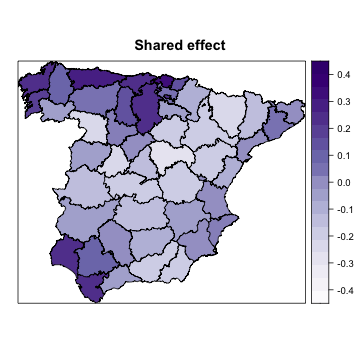
\includegraphics[scale=0.35]{images/Spain_Shared.png}
\includegraphics[scale=0.35]{images/Spain_Esophagus_specific.png}
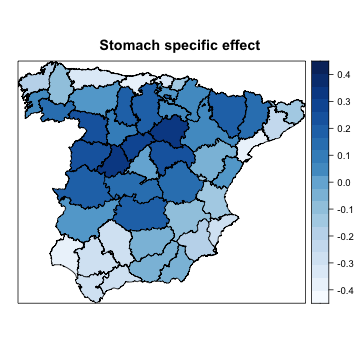
\includegraphics[scale=0.35]{images/Spain_Stomach_specific.png}
\end{center}
\caption{Posterior means of the shared spatial pattern (left), the esophagus-specific spatial pattern (middle) and stomach-specific spatial pattern (right).}
\label{fig:spain}
\end{figure}








\section{Multivariate Continuous Data}
\label{sec:mgeo}


\medskip
Datasets for variables that vary continuously in space contain observations which are geographically referenced, i.e., both the value and where it is collected (e.g., the coordinates) appear in the dataset. Then, the spatial variation of the different variables is estimated using geostatistical models.




\medskip
Similarly to lattice data, geostatistical multivariate models can be fit with \code{R-INLA} by sharing common terms.  Therefore, the first variable can be modelled so that the mean includes a shared spatial term assumed to be a Gaussian process with a covariance defined using a Mat\'ern function, and all the other variables can depend on this shared spatial term plus specific spatial effects. Hence, for example, $D$ variables of interest ($Y_d$ for $d=0, \ldots, D-1$), with a general likelihood function $P(\cdot)$, measured at $n$ different locations can be written as: 

$$
Y_{i,d} \sim P(\mu_{i,d}) .
$$

Then, the mean of the baseline variable ($\mu_{i,0}$) will be modelled as a sum of an intercept ($\alpha_0$) and a shared spatial effect ($u_{i,0}$). Furthermore, the mean of observation $i$ and variable $d$ ($\mu_{i,d}$) will be modeled through an intercept for each variable ($\alpha_d$), the shared spatial effect ($u_{i,0}$) and a specific spatial effect ($u_{i,d}$) as follows:

\begin{align}
\mu_{i,0} =& \alpha_0 + u_{i,0};  &i&=1,\ldots,n\nonumber\\
\mu_{i,d} =& \alpha_k + u_{i,0} + u_{i,d}  &i&=1,\ldots,n;\ d=1,\ldots,D-1\nonumber
\end{align}


\noindent
Here, $u_{i,0}$ represents the shared (between variables) spatial term, while  $u_{i,d}\, (d\geq1)$ represents specific terms that can be used to assess departures from the shared spatial term. These random effect terms are assumed to be Gaussian processes with covariance defined using a Matérn covariance function, which for a generic spatial random effect $u(s)$ is defined as:

$$
Cov(u_p, u_l) = Cov(u(s_p), u(s_l))= \frac{\sigma^2}{\Gamma(\lambda)2^{\lambda-1}} (\kappa \|s_p - s_l\|)^{\lambda}K_{\lambda}(\kappa \|s_p - s_l\|) ,
$$

\noindent
where $\|s_p - s_l\|$ represents the Euclidean distance between points $s_p$ and $s_l$, $\sigma^2$ is the marginal variance of the latent Gaussian process, $\kappa$ is the scaling parameter, which is related to the range, $K_{\lambda}$ represents the modified Bessel function of the second kind, and $\lambda$ is the order term, which measures the smoothness of the process. Furthermore, this latent Gaussian field $u(s)$ can be approximated using the stochastic partial differential equation (SPDE) approach described in \citet{SPDE}. This approach relies on expressing the random effect $u(s)$  as the solution of an SPDE which is approximated through (an appropriate choice of) deterministic basis functions defined in a triangulation of the domain:

$$
u(s) =\sum_{k=1}^{m} \phi_k(s) w_k .
$$

\noindent
Here, $\phi_k(s)$ are the basis functions (pairwise linear functions), $m$ is the total number of nodes (triangle vertices) and $w_k$ are zero-mean Gaussian distributed weights. For more details, the reader is referred to \citet{SPDE}.

\medskip
In this example, all the measurements of the different variables are obtained from the same $n$ locations. However, the measurements of each variable can be from  different locations of the study region. Furthermore, INLA is not able to estimate any cross-covariance using the proposed model as dependence among the variables relies on the shared spatial term. A multivariate geostatistical analysis can be performed using the R package \pkg{gstat}. However, the models implemented in this R package are based on a classic and frequentist  statistical approach.
 


\medskip
Regarding the priors, the SPDE approximation requires setting a prior distribution to the nominal range, $r$, and the nominal standard deviation, $\sigma$. The nominal range is the distance at which the correlation is 0.1. Penalized complexity prior distributions \citep[PC-priors, ][]{PCpriors} can be chosen for both parameters. In a nutshell, PC-priors are based on the idea of penalising the complexity from a simple baseline model (that is, a model in which the parameter has been fixed to a particular reference value), i.e., the prior density is related to the distance from a baseline model. A remarkable benefit of the PC-priors are their high intuitiveness in their definition as they are set by stating values for the probabilities of the parameters, in particular, $P(r < r_0)$ and $P(\sigma > \sigma_0)$ for certain values of $r_0$ and $\sigma_0$.

\medskip
The prior on the range is set such that $r$ is lower than half the maximum distance ($d_m$) between any two points in the study region, with high probability, i.e., $P(r < d_m / 2) \approx 1$. As for the standard deviation, following the example of \citet{Simpson2019Careful} we set an upper  limit $U_\alpha$ such that $\sigma$ is less that this limit with high probability. Therefore, the probability that the standard deviation is greater than this upper limit ($ P(\sigma > U_{\alpha})$) is set to be almost 0.


%\subsection{Geostatistics}

%\medskip
%Geostatistical datasets contain the values of the different variables and the locations where they are measured. In this case, the main objective is to estimate the value of the variables as a continuous surface over the study region. The SPDE \citep{SPDE} will be used in order to analyse the multivariate geostatistical data using a discretization (a mesh) of the surface. 




\subsection{Example: spatial distribution of heavy metals}

The \code{meuse} dataset in the \pkg{gstat} package gives the locations and measurements of topsoil heavy metals collected in a flood plain by the Meuse river close to the village of Stein (located in Netherlands). After loading the \pkg{gstat} package, the data can be loaded using the following code:

\begin{example*}
# Load the data
data(meuse)

# Create the spatial object
coordinates(meuse) <- ~ x + y
proj4string(meuse) <- CRS("+init=epsg:28992")
\end{example*}

These measurements are highly correlated and we will explore in this example how to fit geostatistical models with the SPDE approach. Note that observations do not need to be in a regular grid. Instead of a grid, a mesh is defined to apply the SPDE approach. The boundary of the study region is stored in object \code{meuse.bdy} (see accompanying code). The definition of the mesh is done using the coordinates of the boundary of the area following the code below:

\begin{example*}
# Create the mesh
mesh <- inla.mesh.2d(boundary = meuse.bdy, loc = coordinates(meuse),
  max.edge = c(250, 500), offset = c(250, 500), n = c(32, 32))
\end{example*}

\noindent
The left plot in Figure~\ref{fig:meuse:mesh} shows the mesh built with the above code for this example.



\begin{figure}[h!]
\begin{center}
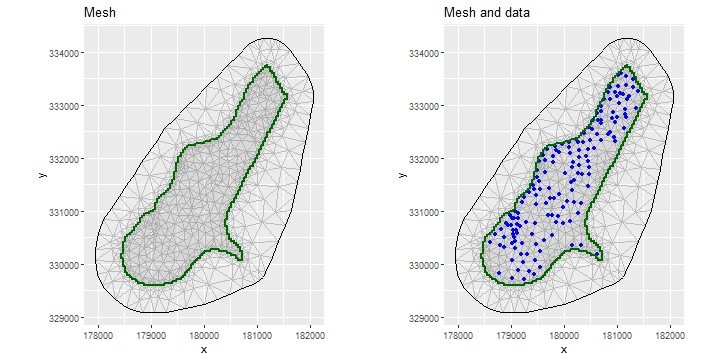
\includegraphics[scale=0.5]{images/meuse_Only2_mesh.png}
\end{center}
\caption{Mesh used in the estimation of the concentration of heavy metals around river Meuse, only with the boundary of the study region (left) and jointly with the survey locations (right).}
\label{fig:meuse:mesh}
\end{figure}

In particular, the model will consider concentrations of lead and zinc. Concentrations have been measured at diferent locations which are displayed in the right plot in Figure \ref{fig:meuse:mesh}. However, data on the concentrations of other metals is also available within the same dataset. Then, a model with all the metal concentrations could be handled following a similar structure. Values (in the original dataset) are considered in the log-scale. These log-transformed concentrations ($\log(y_{l})$ and $\log(y_z)$, respectively) are assumed to be normally distributed. The mean of the log-concentration of lead is modeled using an intercept $\alpha_l$ plus a Gaussian process with a Matérn covariance, $u_{i,s}$, while the mean of the log-concentration of zinc is modeled using an intercept, $\alpha_z$, the shared spatial effect, $u_{i,s}$, plus another spatial Gaussian process with Matérn covariance, $u_{i,z}$. This will allow us to assess differences in the spatial distribution of the concentration of both heavy metals.  Furthermore, the Euclidian distance from the location of each measurement to the closest point of the river ($dist$) is included in both linear predictors as a covariate, each with a different slope parameter ($\beta_l$ and $\beta_z$). 

Hence, the model can be written as: 

$$
\begin{array}{rcl}
\log(y_{l}) &\sim& N(\mu_{i,l}, \sigma_l)\nonumber\\
\log(y_{z}) &\sim& N(\mu_{i,z}, \sigma_z)\nonumber
\end{array}
$$

\noindent
where $\mu_{i,l}$ and $\mu_{i,z}$ represent the mean of the concentration of lead and zinc, respectively and which are modelled as follows:


\begin{align}
\mu_{i,l} =& \alpha_l + \beta_l dist_i + u_{i,s};  &i&=1,\ldots,n\nonumber\\
\mu_{i,z} =& \alpha_z + \beta_z dist_i + u_{i,s} + u_{i,z}  &i&=1,\ldots,n\nonumber
\end{align}


\medskip
In this case, the prior choices for the nominal range ($r$) and standard deviation ($r$) for both the shared and zinc-specific spatial random effects are: 

$$ P(r < 2394.16) = 0.95,  $$
$$ P(\sigma > 1000) = 0.05 .$$

\noindent
%This represents that a nominal range higher than the half of the maximum distance (i.e., 2394.16 meters) of the domain is unlikely. Similarly for the nominal standard deviation, which is really unlikely to be higher than 1000 mg/kg of soil (ppm).
In plain words, this represents the belief that substantial correlations (> 0.1) between points more than half the maximum distance (2394.16 meters) apart are unlikely, and so are standard deviations greater than 1,000. These prior distributions are specified using the \code{inla.spde2.pcmatern()} function:

\begin{example*}
spde <- inla.spde2.pcmatern(mesh = mesh,
  prior.range = c(2394.16, 0.95), prior.sigma = c(1000, 0.05)) 
\end{example*}


The SPDE approximation estimates the spatial random effects at the vertices
of the mesh, so that estimates at any other point are based on the estimates at the vertices of the triangle that contains the point. The position of this point inside the triangle is identified
using barycentric coordinates \citep[see][for details]{Krainskietal:2019}.
The projector matrix contains all these coordinates for all the points in the
dataset and it is obtained with function \code{inla.spde.make.A()}:

\begin{example*}
A.m <- inla.spde.make.A(mesh = mesh, loc = coordinates(meuse))
\end{example*}



\medskip
In order to fit models using the SPDE approach, data must be \textit{stacked} using the appropriate format. Helper function \code{inla.stack()} can be used to build a \code{stack} object which contains the data (properly structured), the effects considered in the model, and the projector matrix. Specifically, a \code{stack} object will be built to model each variable. Then, all these objects will be put together into a single \code{stack} object so that a joint model can be fit.

\medskip
In all the stacks the name of the response variable will be the same. The values will be given in a matrix with as many columns as the number of variables and as many rows as the number of observations. In the first stack, the values of the first response variable will be in the first column and the rest of columns will be filled with \code{NA}'s. The other stacks and corresponding response variables will be defined analogously.


\medskip
Regarding fixed and other latent effects included in the linear predictor, these can take
the same name across stacks when the effect is shared for different
response variables. When the effect of the same covariate or latent effect
needs to be different across response variables, then different names must be used. See the R code below for more details.



%ESTO HAY QUE REVISARLO PORQUE CREO QUE NO SE CORRESPONDE CON EL CÓDIGO.
%
%
%
%\medskip
%\textcolor{red}{
%Instead of using a single matrix to pass the values of the response variables (as in the multivariate lattice example),
%each column of the matrix will be passed together with all the other 
%variables required to model the distribution of each heavy metal. The measured values of each variable will be included in its stack using a vector which will follow the same structure as in the multivarite lattice data example. As a general example, let's consider $K$ variables and $n$ observations. In this case, all the vectors will have $K \times n$ length and, for instance, the vector of the stack of the first variable will store the $n$ values of the first component and the rest will be filled with \code{NA}'s.}
%
%\medskip
%\textcolor{red}{As a toy example, let's consider $K=3$ and $n=2$, and the values of the three variables which are stored in this matrix:}
%
%\textcolor{red}{
%$$
%\begin{bmatrix}
%1.2 & 4.8 & 3.7 \\
%2.1 & 6.5 & 5.4
%\end{bmatrix}
%$$
%}
%
%\textcolor{red}{The three vectors (each will be placed in the corresponding stack) are:}
%
%$$
%[1.2, 2.1, NA, NA, NA, NA]^{\top}, 
%[NA, NA, 4.8, 6.5, NA, NA]^{\top},
%[NA, NA, NA, NA, 3.7, 5.4]^{\top}
%$$

\medskip
The data are structured using the \code{inla.stack()} function specifying three elements: the data, the projector matrix, the different effects of the linear predictor and a tag to identify each part of the dataset in the final stack. This tag is used when retrieving particular results from the output.

\begin{example*}
# Create the stack object for lead
stk.lead <- inla.stack(
  data = list(log.y = cbind(log(meuse$lead), NA)),
  A = list(A.m, 1),
  effects = list(spatial.field.lead = 1:spde$n.spde,
    data.frame(Intercept.lead = 1, dist.lead = meuse$dist)),
  tag = "Lead")

# Create the stack object for zinc
stk.zinc <- inla.stack(
  data = list(log.y = cbind(NA, log(meuse$zinc))),
  A = list(A.m, A.m, 1),
  effects = list(
    spatial.field.zinc = 1:spde$n.spde, base.copy.zinc = 1:nv,
    data.frame(Intercept.zinc = 1, dist.zinc = meuse$dist)),
  tag = "Zinc")
\end{example*}

A projector matrix and a stack for the prediction grid have also been created as follows:

\begin{example*}
# Create the projector matrix for the prediction
A.pr <- inla.spde.make.A(mesh = mesh, loc = coordinates(meuse.grid))

# Prepare the data for the prediction
y.pred <- matrix(NA, nrow = nrow(meuse.grid), ncol = 2)

# Build predicting stack for lead
stk.lead.pr <- inla.stack(
  data = list(log.y = y.pred),
  A = list(A.pr, 1),
  effects = list(spatial.field.lead = 1:spde$n.spde,
    data.frame(Intercept.lead = 1, dist.lead = meuse.grid$dist)),
  tag = "Lead.pred")

# Build predicting stack for zinc
stk.zinc.pr <- inla.stack(
  data = list(log.y = y.pred),
  A = list(A.pr, A.pr, 1),
  effects = list(
    spatial.field.zinc = 1:spde$n.spde, base.copy.zinc = 1:nv,
    data.frame(Intercept.zinc = 1, dist.zinc = meuse.grid$dist)),
  tag = "Zinc.pred")

\end{example*}

Next, a \code{stack} object is built for the shared and zinc-specific effects in order to study the spatial patterns of these effects: 

\begin{example*}

# Stack for the shared effect
stk.shared <- inla.stack(
  data = list(log.y = y.pred),
  A = list(A.pr),
  effects = list(spatial.field.lead = 1:spde$n.spde),
  tag = "Shared")

# Stack for the specific sp effect zinc
stk.zinc.spec <- inla.stack(
  data = list(log.y = y.pred),
  A = list(A.pr),
  effects = list(spatial.field.zinc = 1:spde$n.spde),
  tag = "Zinc.spec")
\end{example*}

All the \code{stack} objects are put together in a single joint \code{stack} object using the \code{inla.stack()} function: 

\begin{example*}
# Put all the stacks together
join.stack <- inla.stack(
  stk.lead, stk.zinc, 
  stk.zinc.pr, stk.lead.pr,
  stk.shared, stk.zinc.spec)
\end{example*}

The model formula is defined below. The latent effect of type \code{copy} is used to define the shared term of the model. 

\begin{example*}
# Formulas for the model
form <- log.y ~ -1 + Intercept.lead + Intercept.zinc + dist.lead + dist.zinc + 
  f(spatial.field.lead, model = spde) +
  f(spatial.field.zinc, model = spde) + 
  f(base.copy.zinc, copy = "spatial.field.lead", fixed = TRUE)  

\end{example*}

Finally, the model is fit with \pkg{R-INLA}. Note how the \code{family} argument takes a vector of two \code{"gaussian"} elements (one for each heavy metal concentration). Furthermore, note that the data are obtained from the joint stack with the \code{inla.stack.data()} function and that the projector matrix \code{A} is also obtained using the \code{inla.stack.A()} function. 

\begin{example*}
meuse.res <- inla(formula = form, verbose = FALSE, 
  data = inla.stack.data(join.stack, spde = spde),
  family = rep("gaussian", 2), 
  control.family = list(zero.prec, zero.prec),
  control.predictor = list(A = inla.stack.A(join.stack), compute = TRUE),
  control.compute = list(dic = TRUE, waic = TRUE, cpo = TRUE, mlik = TRUE, po = TRUE))
\end{example*}

Given that the structure of the data used for model fitting is a \code{stack} now, particular parameter estimates can be accessed through function \code{inla.stack.index()}. This function can provide the indices to access the entries of
specific data or latent effects in the summaries provided by \pkg{R-INLA}. For example, the following code can be used to obtain the posterior means of the fitted values obtained with the effects in the \code{'Lead.pred'} stack:

\begin{example*}
idx.lead <- inla.stack.index(join.stack, 'Lead.pred')$data
meuse.grid$lead.pr <- meuse.res$summary.fitted.values[idx.lead, 'mean']
\end{example*}

Figure~\ref{fig:meuse:est} shows point estimates (posterior means) of the log-concentration of lead and zinc; the posterior mean of the shared and the zinc-specific effect are also shown. Note the similar spatial pattern across both metals.



\begin{figure}[h!]
\begin{center}
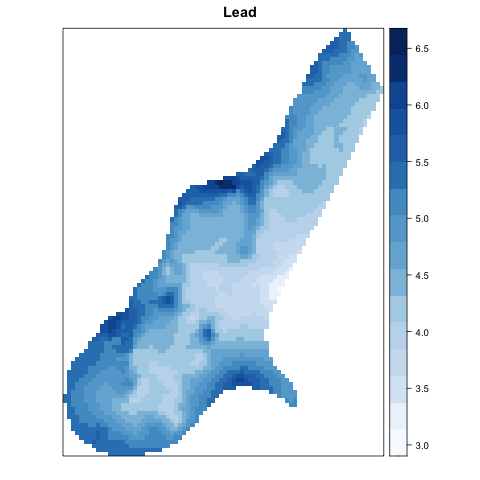
\includegraphics[scale=0.35]{images/Meuse_lead_estimate.png}
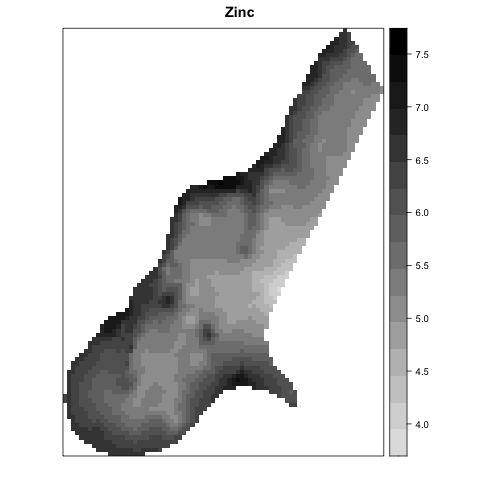
\includegraphics[scale=0.35]{images/Meuse_zinc_estimate.png}
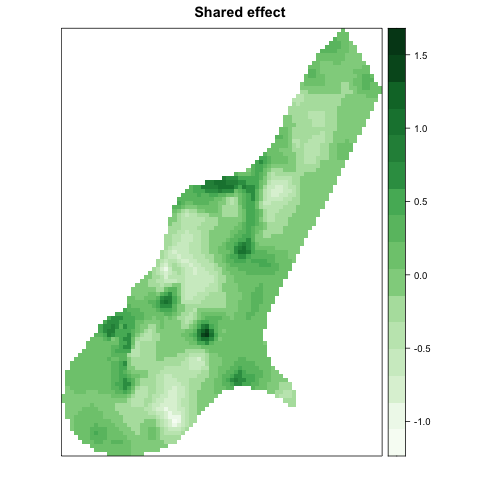
\includegraphics[scale=0.35]{images/Meuse_Shared_effect.png}
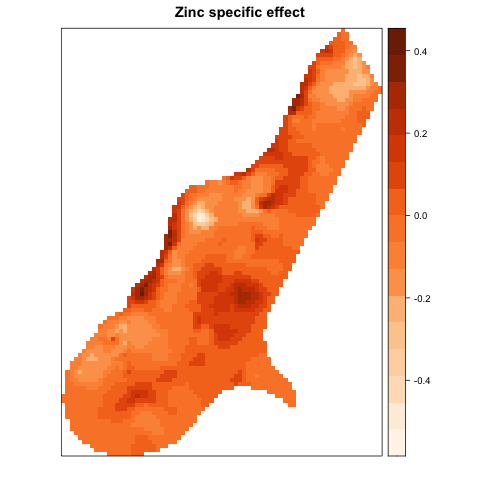
\includegraphics[scale=0.35]{images/Meuse_Zinc_specific.png}
\end{center}
\caption{Estimates of the posterior means of the log-concentration of lead (top-left) and zinc (top-right). Estimates of the posterior mean of the shared spatial effect (bottom-left) and the zinc-specific spatial effect (bottom-right).}
\label{fig:meuse:est}
\end{figure}





\section{Multivariate point patterns}
\label{sec:mpp}

\medskip
A point pattern is defined as a group of points (geographically located) which are a single realization of a stochastic process called point process. A multivariate point pattern can be defined as a group of several point patterns where each point pattern has a different origin, i.e., each point pattern is caused by different processes. These are also referred to a specific case of \textit{marked} point pattern \citep{spatstat:2015} where each point pattern is labelled with a categorical mark.

In a completely random point process, points appear independently of each other and uniformly over the study region. This is also known as a homogeneous Poisson process with (constant) intensity $\lambda$, which measures the average number of points per unit area. It is also possible to consider a spatially varying intensity, $\lambda(s)$ (with $s$ being a point of the study region), so that the process becomes an \textit{inhomogeneous} Poisson process. The model can be extended to more complex point patterns \citep[see, for example,][]{spatstat:2015}.

Several methods have been used to model the intensity function $\lambda(s)$. A complete spatial randomness scenario will not be considered here, that is, the intensity function of each point pattern will not be considered as constant over the study area. Specifically, intensities will be considered as continuous processes over the entire study region and they will be modeled using log-Gaussian Cox processes \citep{Moller,DiggleMoraga}. Log-Gaussian Cox processes can be fit by including spatial terms using the SPDE approach implemented in INLA \citep{Simpsonetal:2016}. The analysis of the intensity as a continuous function over the study region is similar to the case of multivariate geostatistics.

\medskip
Given $K$ point patterns in a region $\mathcal{D}$, an example of how to structure a multivariate point patterns model is: 


\begin{align*}
\log(\lambda_{0}(s)) =& \alpha_0 + u_{0}(s);  &s&\in \mathcal{D}\\
\log(\lambda_{j}(s)) =& \alpha_j + u_{0}(s) + u_{j}(s)  &s&\in \mathcal{D};\ j=1,\ldots,K-1\nonumber
\end{align*}
\noindent
where $\lambda_{0}(s)$ is the intensity of the baseline point pattern and $\lambda_{j}(s)$ the intensity function of the $j$th point pattern. Moreover, $\alpha_0,\alpha_j$ terms represent the intercepts and $u_0(s), u_j(s)$ are the spatial effects. Specifically, $u_0(s)$ is the shared (by the different point patterns) spatial term and $u_j(s)$ are the specific spatial terms which model the differences between each point pattern and the baseline. 

\medskip
In spatial epidemiology, the goal is often to discern whether a distribution of cases follows the spatial distribution of a set of controls, or whether it depends on exposure to pollution sources or other risk factors such as pollution \citep{PalmiPerales2019Biometrical}. This is an application of the model described here, in which the log-intensity of the controls can be modeled using a shared spatial term and the log-intensity of the cases can include this shared spatial term plus a disease-specific spatial term. Furthermore, the linear predictor can include other terms to account for risk factors.

\medskip
Priors are set similarly as in the example for continuous spatial data as the spatial random effects $u_j(s),\ j=0,\ldots,K-1$ are actually modeled as SPDE latent effects. Other parameters of effects included in the model (e.g., fixed effects) will be asssigned priors accordingly.
 

\subsection{Example: forest fires in Castilla-La Mancha (Spain)}
\label{exam:mpp}


\medskip
The \pkg{spatstat} package contains the \code{clmfires} dataset. This dataset records the occurrence of forest fires in the region of Castilla-La Mancha (Spain) from 1998 to 2007. These forest fires are classified by four different causes: lightning, accidental, intentional, and other fires (Figure \ref{fig:clmfires:data}). After loading the packages, the data are accessed using the \code{data()} function:

\begin{example*}
#Load and display the data
data("clmfires")
\end{example*}

Specifically, in this example, the intensities of the different types of forest fires are estimated by considering lightning fires as the baseline pattern. Furthermore, INLA is used to assess the similarities or differences among their spatial patterns. First of all, the mesh is built using the coordinates of the boundary of the dataset (\code{bdy.SP}) using the code below.

\begin{example*}
mesh <- inla.mesh.2d(
  boundary = list(bdy.SP, NULL), cutoff = 2, max.edge = c(20, 50),
  min.angle = 27, offset = c(1, 50), n=c(16,16))
\end{example*}



\begin{figure}[h!]
\begin{center}
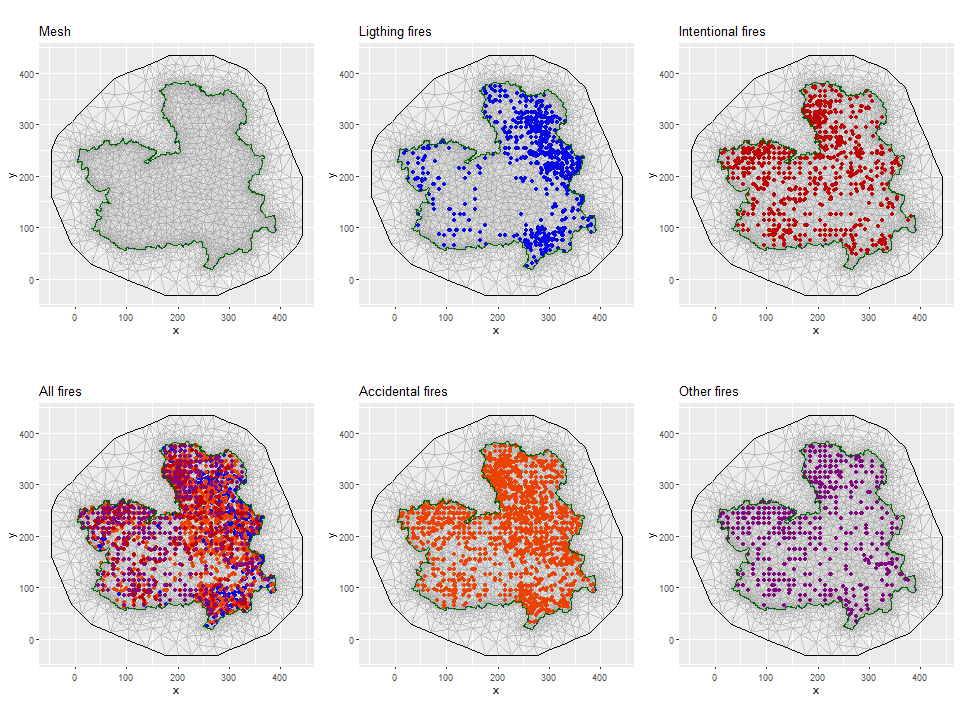
\includegraphics[scale=0.40]{images/clmfires_mesh.png}
%\includegraphics[scale=0.5]{chorley_est_spatial.pdf}
\end{center}
\caption{The mesh used is shown alone (top-left) and with all the fire types (bottom-left). Furthermore, the mesh is also displayed for each fire type separately: lightning fires (top-middle), accidental fires (bottom-middle), intentional fires (top-right), and other fires (bottom-right).}
\label{fig:clmfires:data}
\end{figure}	 


Following the model structure for multivariate point patterns detailed above, the log-intensity of the lightning fires $\lambda_l(s)$ will be modeled using an intercept, $\alpha_l$, and a spatial Gaussian effect with Mat\'ern covariance, $u_l(s)$ as follows 

$$\log{\lambda_l(s)}= \alpha_l + u_l(s); \,\,\, s\in D$$  

Spatial effect $u_l(s)$ will also be shared in the linear predictor of the other types of fire. Similarly, the log-intensity of the accidental, intentional, and other fires (which includes unknown cause) will be modeled using specific intercepts, plus the shared spatial effect, plus a specific spatial effect as follows: 

$$\log{\lambda_a(s)}= \alpha_a + u_l(s) + u_a(s); \,\,\, s\in D $$ 
$$\log{\lambda_i(s)}= \alpha_i + u_l(s) + u_i(s); \,\,\, s\in D $$  
$$\log{\lambda_o(s)}= \alpha_o + u_l(s) + u_o(s) \,\,\, s\in D $$  
 
\noindent
Following the prior specification section, the chosen PC-priors in this example are:


$$ P(r < 200) = 0.95$$
$$ P(\sigma > 100) = 0.05 $$

\noindent
where a nominal range higher than half the maximum distance (e.g., 200 kilometres) of the domain is unlikely. Similarly for the nominal standard deviation, its prior assumes that it is really unlikely that it is higher than 100 in this context. These prior distributions have been specified using function \code{inla.spde2.pcmatern()}:

\begin{example*}
spde <- inla.spde2.pcmatern(mesh = mesh,
  prior.range = c(200, 0.95),  prior.sigma = c(10, 0.05)) 
\end{example*}

\noindent
Here, argument \code{prior.range} sets the prior for the range and the argument \code{prior.sigma} sets the prior for the standard deviation of the spatial effect. 

\medskip
As this model includes SPDE latent effects, data must be put together using \code{stack} objects. In the case of point patterns, the data included in the stack function is different from the geostatistical example as point pattern data has to be detailed following a specific structure (see below). Model fitting now relies on the methods described in \cite{Simpsonetal:2016}. In this case, two elements will be included in a list for storing the data of each point pattern.

\medskip
The first element of the list will be a matrix with $N_v + N_i$ rows and $K$ columns where $N_v$ is the number of vertices of the SPDE mesh, $N_i$ is the total number of points of the $i$-th point pattern and $K$ is the number of different point patterns. The matrix of the stack of the $i$-th point pattern will be filled with \code{NA}'s except for the $i$-th column. This $i$-th column will contain firstly $N_v$ zeros corresponding to the points of the mesh. After these zeros, there will be $N_i$ ones corresponding to the $N_i$ points of the $i$-th point pattern.

\medskip
The second element of the list will be a vector containing an offset. Specifically, the length of this vector is also $N_v + N_i$ where the first $N_v$ elements will contain the "weights" of the mesh points. The reader is referred to \citet{Simpsonetal:2016} for more details about this approximation. The rest of the values will be zeros.

\medskip
These two elements have to be created for each stack of each point pattern. Then, as before, the stacks are combined in a single stack object. As a toy example, consider a mesh with $N_v =3$, two point patterns ($K=2$) with three and four points, respectively ($N_1=3$ and $N_2=4$). The weights associated to the three mesh points will be 2.3, 4.3 and 6.2. Then, the data passed to the first and second stack are:


$$ 
\begin{bmatrix}
0 & \texttt{NA}\\
0 & \texttt{NA}\\
0 & \texttt{NA}\\
1 & \texttt{NA}\\
1 & \texttt{NA}\\
1 & \texttt{NA}
\end{bmatrix},
\begin{bmatrix}
2.3\\
4.3\\
6.2\\
0\\
0\\
0
\end{bmatrix}; \ \ \ 
\begin{bmatrix}
\texttt{NA} & 0  \\
\texttt{NA} & 0  \\
\texttt{NA} & 0  \\
\texttt{NA} & 1  \\
\texttt{NA} & 1  \\
\texttt{NA} & 1  \\
\texttt{NA} & 1  
\end{bmatrix}, 
\begin{bmatrix} 
2.3\\
4.3\\
6.2\\
0\\
0\\
0\\
0
\end{bmatrix} .
$$


As stated above, when analysing point patterns it is necessary to assign some
weights to the points of the mesh. This is done by creating a Voronoi
tesselation using these points, so that the area of the associated polygon
becomes the associated weight. The following code illustrates how to obtain the
Voronoi tesselation and the associated weights:
 
\begin{example*}
library(deldir)
dd <- deldir(mesh$loc[, 1],mesh$loc[, 2])
# Create a list of tiles in a tessellation
mytiles <- tile.list(dd)

# Boundary as a polygon
pl.study <- as(bdy, "gpc.poly")
# Area of the study area
area.poly(pl.study)

# Compute weights as the area of the polygon given as an
# intersection between Voronoi tiles and domain polygon
w <- unlist(lapply(mytiles,
  function(p) area.poly(
    intersect(as(cbind(p$x,p$y), "gpc.poly"), pl.study)
    )
  )
)
\end{example*}

These computed weights are introduced as the expected weights on the mesh points. Furthermore, the data should be structured as follows:

\begin{example*}
# Data for the stack function: lightning fires
e.lig <- c(w, rep(0, n.lig))
y.lig <- matrix(NA, nrow = nv + n.lig, ncol = n.pp)
y.lig[, 1] <- rep(0:1, c(nv, n.lig))

# Data for the stack function: accidental fires
e.acc <- c(w, rep(0, n.acc))
y.acc <- matrix(NA, nrow = nv + n.acc, ncol = n.pp)
y.acc[, 2] <- rep(0:1, c(nv, n.acc))

# Data for the stack function: intentional fires
e.int <- c(w, rep(0, n.int))
y.int <- matrix(NA, nrow = nv + n.int, ncol = n.pp)
y.int[, 3] <- rep(0:1, c(nv, n.int))

# Data for the stack function: other fires
e.oth <- c(w, rep(0, n.oth))
y.oth <- matrix(NA, nrow = nv + n.oth, ncol = n.pp)
y.oth[, 4] <- rep(0:1, c(nv, n.oth))
\end{example*}

Another element of the SPDE approach is the projector matrix that represents each point using barycentric coordinates from the mesh points (as explained above). When analysing multivariate point patterns, this matrix has two parts: one for the mesh points (named \code{imat}), which is a diagonal matrix as every mesh point matches itself when using barycentric coordinates, and the other for the points of the point pattern (named \code{lmat}). Then, the projector matrix is the combination of these two matrices:

\begin{example*}
#imat: define imat
imat <- Diagonal(nv, rep(1, nv))

#lmat: define lmat
lmat.lig <- inla.spde.make.A(mesh, pts.lig)
lmat.acc <- inla.spde.make.A(mesh, pts.acc)
lmat.int <- inla.spde.make.A(mesh, pts.int)
lmat.oth <- inla.spde.make.A(mesh, pts.oth)

#Projector matrix: Put together imat and lmat
A.lig <- rbind(imat, lmat.lig)
A.acc <- rbind(imat, lmat.acc)
A.int <- rbind(imat, lmat.int)
A.oth <- rbind(imat, lmat.oth)
\end{example*}

Once all the elements of the \code{stack} object are set, the \code{inla.stack()} function is used to build the different \code{stack} objects. For instance, the \code{stack} objects of two (out of four) types of forest fires are shown here below:

\begin{example*} 
# Create the stack for the lighting fires
stk.lig <- inla.stack(
  data = list(y = y.lig, e = e.lig),
  A = list(A.lig, 1),
  effects = list(spatial.field.lig = s.index.lig, 
    data.frame(Intercept.lig = rep(1, n.lig)) 
    ),
  tag = "Lighting")

# Create the stack for the accidental fires
stk.acc <- inla.stack(
  data = list(y = y.acc, e = e.acc), 
  A = list(A.acc, A.acc, 1), 
  effects = list(
    base.copy.acc = 1:nv, 
    spatial.field.acc = s.index.acc, 
    data.frame(Intercept.acc = rep(1, n.acc))
    ),
  tag = "Accidental")
\end{example*}

As in the example for continuous spatial data, the \code{stack} objects for the predictions have to be built following the same structure (their name will end with ".pr" in the R code). Finally, all the \code{stack} objects are joined into a single joint \code{stack} object as follows: 

\begin{example*}

# All stacks together
join.stack <- inla.stack(
  stk.lig, stk.acc, stk.int, stk.oth, 
  stk.lig.pr, stk.acc.pr, stk.int.pr, stk.oth.pr, 
  stk.shared, stk.acc.spec, stk.int.spec, stk.oth.spec)

\end{example*}

\noindent
Note that in this example separate \code{stack} objects have been created for estimating the intensity of each of the different types of forest types,  the shared spatial pattern (stack \code{stk.shared}) and the three different specific spatial effects (stacks \code{stk.acc.spec}, \code{stk.int.spec} and \code{stk.oth.spec}). 

The model formula is defined here below, where the latent effects of type
\code{copy} are used to define the shared terms of the model: 

\begin{example*} form <- y ~ -1 + Intercept.lig + Intercept.acc + Intercept.int + Intercept.oth +
  f(spatial.field.lig, model = spde) +
  f(spatial.field.acc, model = spde) + 
  f(base.copy.acc, copy = "spatial.field.lig", fixed = TRUE) +
  f(spatial.field.int, model = spde) + 
  f(base.copy.int, copy = "spatial.field.lig", fixed = TRUE) +
  f(spatial.field.oth, model = spde) + 
  f(base.copy.oth, copy = "spatial.field.lig", fixed = TRUE)    

\end{example*}

The model is fit with \pkg{R-INLA} using the code below. Note how the \code{family} argument takes a vector of four \code{"poisson"} elements (one for each fire type). 

\begin{example*}
pp.res <- inla(formula = form, verbose = FALSE, 
  data = inla.stack.data(join.stack, spde = spde), 
  family = rep("poisson", 4), 
  control.predictor = list(A = inla.stack.A(join.stack), compute = TRUE, link = 1),
  control.compute = list(dic = TRUE, waic = TRUE, cpo = TRUE, mlik = TRUE, po = TRUE)
)
\end{example*}

Figure~\ref{fig:clmfires:est1} shows the posterior mean of the intensity of each type of the forest fires. A different spatial pattern can be seen for each fire type. Lightning fires mostly appear in the east part of the region, while the other three types of forest fires are more likely to appear in the west and the central parts of the region. Additionally, the posterior means of the shared and specific spatial effects can also be seen in Figure~\ref{fig:clmfires:est2}. 

\begin{figure}[h!]
\begin{center}
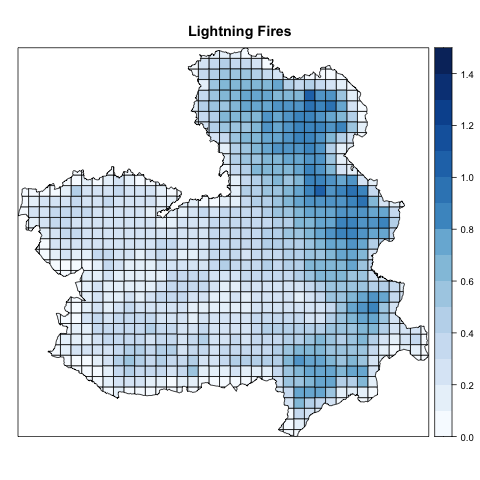
\includegraphics[scale=0.40]{images/CLMFires_lightning.png}
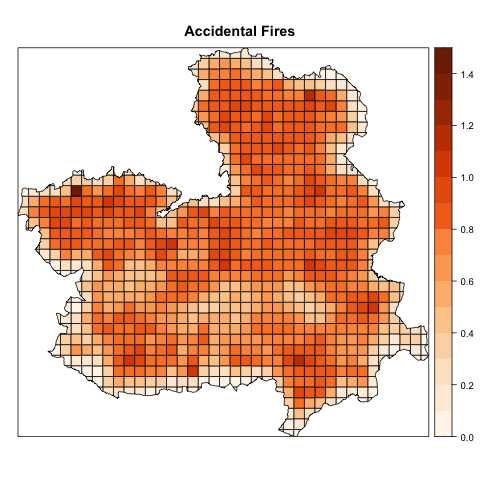
\includegraphics[scale=0.40]{images/CLMFires_accidental.png}
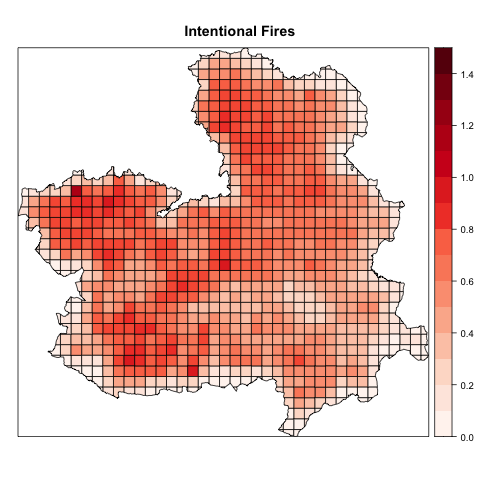
\includegraphics[scale=0.40]{images/CLMFires_intentional.png}
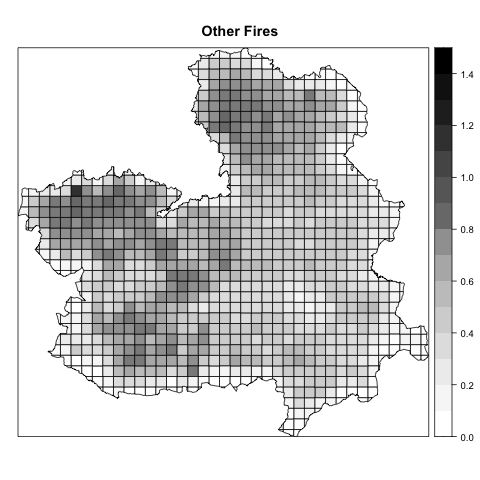
\includegraphics[scale=0.40]{images/CLMFires_other.png}
\end{center}
\caption{Posterior mean of the intensity of the lightning (top-left), accidental (top-right), intentional (bottom-left) and other (bottom-right) fires.}
\label{fig:clmfires:est1}
\end{figure}

\begin{figure}[h!]
\begin{center}
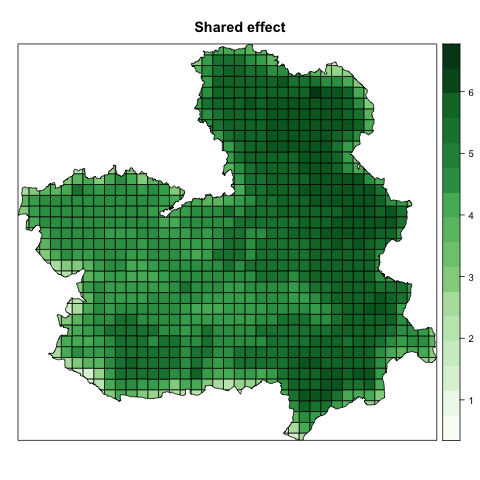
\includegraphics[scale=0.40]{images/CLMFires_shared.png}
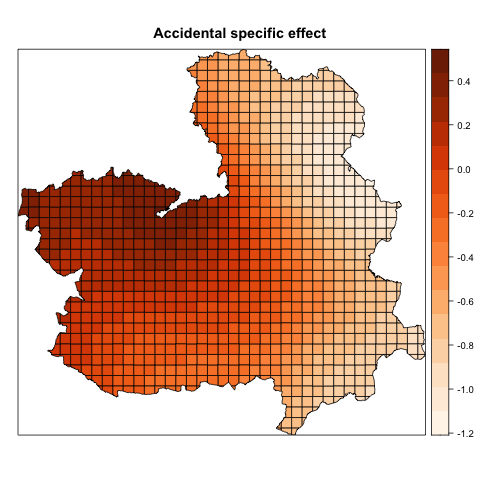
\includegraphics[scale=0.40]{images/CLMFires_acc_specific.png}
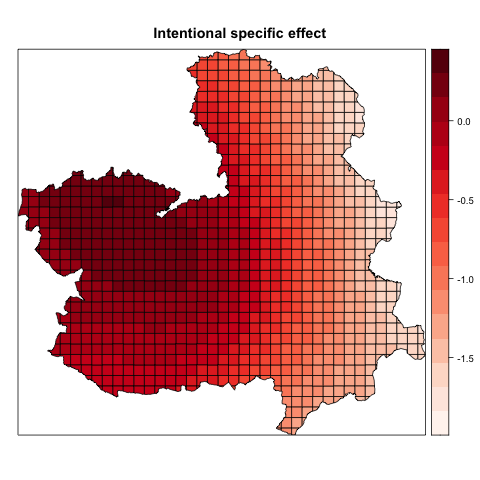
\includegraphics[scale=0.40]{images/CLMFires_int_specific.png}
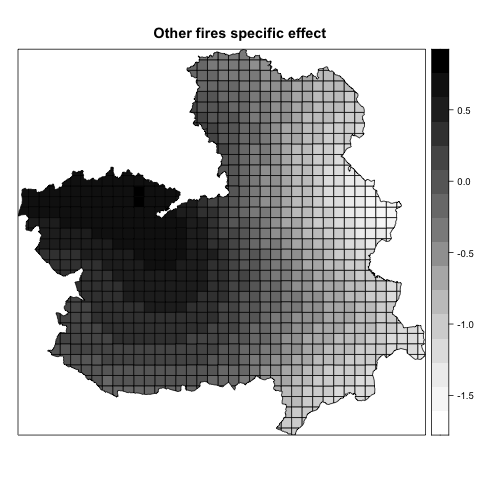
\includegraphics[scale=0.40]{images/CLMFires_Other_specific.png}
\end{center}
\caption{Posterior mean of the shared spatial effect (top-left), the accidental-specific (top-right), the intentional-specific (bottom-left) and the other-specific (bottom-right) spatial effects.}
\label{fig:clmfires:est2}
\end{figure}


\section{Discussion}
\label{sec:dis}

\medskip
In this paper, we have shown how to fit multivariate spatial models using the \pkg{R-INLA} package. In particular, the details of how to analyse each spatial data type (lattice, continuous, and point patterns) have been given. Furthermore, we have illustrated the application of these models using three datasets: simulated data on mortality by three types of cancer (available from \url{https://github.com/becarioprecario/INLAMCMC_spatial_examples}), the \code{clmfires} dataset in the \pkg{spatstat} package and the \code{meuse} dataset in the \pkg{gstat} package. Furthermore, more complex spatial and spatio-temporal models to multivariate data can be fitted with \pkg{R-INLA} \cite[see, for example,][]{INLAMSM}.

\medskip
The main goal of this work has been to illustrate how to perform multivariate spatial Bayesian inference using \pkg{R-INLA}. In particular, we have paid attention to the different steps required to create the necessary data structures for model fitting. The advantage of \pkg{R-INLA} compared with alternatives is its computational efficiency; particularly, MCMC-based methods can struggle in the computationally demanding high-dimensional setting of spatial data sets. Hence, it has been shown that \pkg{R-INLA} is a useful and a worthwhile toolbox for fitting multivariate spatial models. Additionally, the necessary R scripts to reproduce the examples are available at \url{https://github.com/FranciscoPalmiPerales/Mult-Sp-INLA}. 


\section{Acknowledgements}

This work has been supported by grants SBPLY/17/180501/000491 and SBPLY/21/180501/000241, funded by Consejer\'ia de Educaci\'on, Cultura y Deportes (JCCM, Spain) and Fondo Europeo de Desarrollo Regional, grant MTM2016-77501-P and PID2019-106341GB-I00, funded by Ministerio de Econom\'ia y Competitividad (Spain), grants PID2019-106341GB-I00 and PID2022-136455NB-I00, funded by Ministerio de Ciencia e Innovaci\'on (Spain), and grant  CIAICO/2022/165, funded by Dirección General de Ciencia e Investigación (Generalitat Valenciana).  F. Palm\'i-Perales was supported by a doctoral scholarship awarded by the University of Castilla–La Mancha (Spain) and by grant PID2021-128228NB-I00 funded by Ministerio de Ciencia e innovaci\'on. 





